\documentclass[10pt]{article}
\PassOptionsToPackage{hyphens}{url}
\usepackage{hyperref}
\usepackage[margin=0.75in]{geometry}

\usepackage{multicol}
\usepackage{textcomp}
\usepackage{color}
\usepackage{graphicx}
\definecolor{pblue}{rgb}{0.13,0.13,1}
\definecolor{pgreen}{rgb}{0,0.5,0}
\definecolor{pred}{rgb}{0.9,0,0}
\definecolor{pgrey}{rgb}{0.46,0.45,0.48}

\usepackage{listings}
\lstdefinestyle{term}{language=bash,
  columns=fullflexible,
  showspaces=false,
  showtabs=false,
  breaklines=true,
  showstringspaces=false,
  tabsize=2,
  breakatwhitespace=true,
  commentstyle=\color{pgreen},
  keywordstyle=\color{pblue},
  stringstyle=\color{pred},
  basicstyle=\small\ttfamily,
  frame=single,
  moredelim=[il][\textcolor{pgrey}]{$$},
  moredelim=[is][\textcolor{pgrey}]{\%\%}{\%\%},
  upquote=true
}
\lstdefinestyle{sh}{language=bash,
  columns=fullflexible,
  showspaces=false,
  showtabs=false,
  breaklines=true,
  showstringspaces=false,
  tabsize=2,
  breakatwhitespace=true,
  commentstyle=\color{pgreen},
  keywordstyle=\color{pblue},
  stringstyle=\color{pred},
  numbers=left,
  stepnumber=1,
  basicstyle=\small\ttfamily,
  frame=single,
  moredelim=[il][\textcolor{pgrey}]{$$},
  moredelim=[is][\textcolor{pgrey}]{\%\%}{\%\%},
  upquote=true
}

\lstdefinestyle{py}{language=python,
  columns=fullflexible,
  showspaces=false,
  showtabs=false,
  breaklines=true,
  showstringspaces=false,
  tabsize=2,
  breakatwhitespace=true,
  commentstyle=\color{pgreen},
  keywordstyle=\color{pblue},
  stringstyle=\color{pred},
  numbers=left,
  stepnumber=1,
  basicstyle=\small\ttfamily,
  frame=single,
  moredelim=[il][\textcolor{pgrey}]{$$},
  moredelim=[is][\textcolor{pgrey}]{\%\%}{\%\%},
  upquote=true
}

\lstdefinestyle{txt}{
  columns=fullflexible,
  showspaces=false,
  showtabs=false,
  breaklines=true,
  showstringspaces=false,
  tabsize=2,
  breakatwhitespace=true,
  numbers=left,
  stepnumber=1,
  basicstyle=\small\ttfamily,
  frame=single,
  moredelim=[il][\textcolor{pgrey}]{$$},
  moredelim=[is][\textcolor{pgrey}]{\%\%}{\%\%},
  upquote=true
}

\usepackage[T1]{fontenc}

\title{\textbf{Week 03} \\
ssh, grep, regexes, if, and bash scripts
}
\author{
	Melvyn Ian Drag
}
\date{\today}


\begin{document}
\maketitle

\begin{abstract}
Tonight we'll look at grep a bit more, we'll learn what a regex is, youll see
how if statements work in bash, we'll see a tidy way to write bash commands, and
you'll use a cool tool called ssh.
\end{abstract}

\section{ssh}
Let's start with the coolest thing. We'll make a remote connection to a remote
pc. At my house I have a raspberry pi running. 

{\LARGE \textbf{Now connect to the pc using ssh from the command line. And poke
around a bit. Class should think it's cool}}

Now I want you to do the same thing. To do this you need an ssh key. To get a
key you open git bash, a linux terminal or a mac terminal. Type `ssh-keygen' and
then just hit yes to everything. \textbf{Show the class how to do this using git
bash }. Then:

\begin{lstlisting}[style=term]
mel@laptop$ cd 
mel@laptop$ pwd
/home/mel/
mel@laptop$ ls -a
.. lots of stuff including a .ssh directory
mel@laptop$ cd .ssh
mel@laptop$ ls 
id_rsa id_rsa.pub
mel@laptop$ cat id_rsa.pub
A LOT OF STUFF
\end{lstlisting}

Now I want you to be able to connect to my raspberry pi

I need everyone to get me his or her id\_rsa.pub.

Actually have everyone email me the id\_rsa.pub file.


Then Im going to do some magic on my end and you'll be able to connect ot my
computer. We have alot to cover today so go fast, get this done, I don't want
this to take the whole class!

(Add the keys to the homeserver and then the students can connect to my
raspberry pi)

\begin{figure}[h]
\centering
	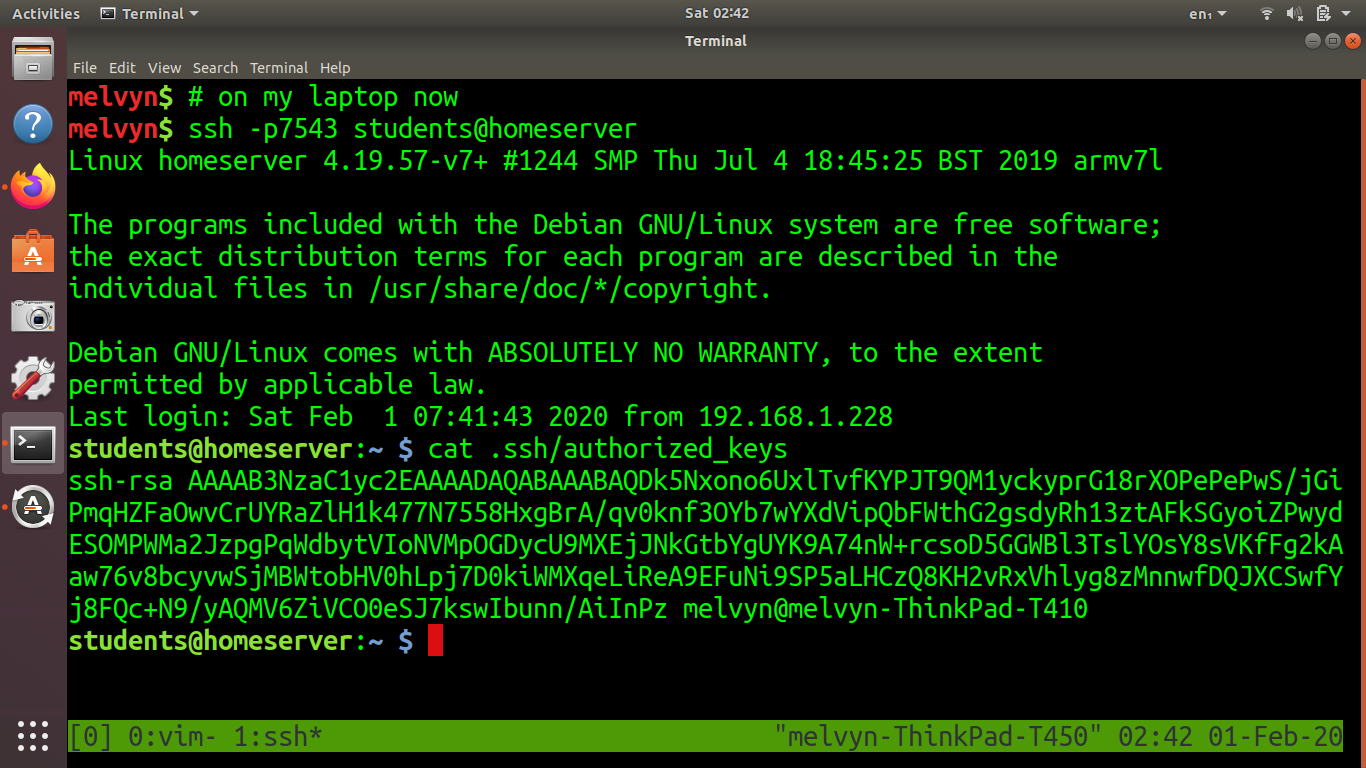
\includegraphics[width=0.8\textwidth]{Images/sshToHomeserver.png}
	\caption{I need to add your ssh key to my authorized\_keys file so you can
connect to my raspberry pi}
	\label{fig:firstssh}
\end{figure}


To connect you'll need to type

\begin{lstlisting}[style=term]
student@njcuPC$ ssh -p 7543 students@72.76.164.224
\end{lstlisting}

and then you should see your prompt change to 

\begin{lstlisting}[style=term]
students@homeserver$
\end{lstlisting}

you're now connected to a computer I have at home using a tool called ssh! There
are some commands that haven't worked in git bash yet like lsblk, wget and man
because those are linux only commands - if you try them now, you'll see they
work

{\LARGE WARNING! I don't know if my server can support 25 people logging in.
This might fail for some, or the computer might work painfyully slow. This is a
server I set up and didn't configure, I don't know what hte default params are.
you can limit the number of remote connections, and the raspberry pi is a small,
humble machine, it probably will cry when 25 ppl try to work on it
simultaneously. Let's see, I've never tried this before! Right now if you were a
hacker you would probably be able to do damage to me because I've allowed you
into my jome network, but I don't think anyone here knows enough yet to do me
any damage.}

Try downloading something with wget:

\begin{lstlisting}
student@homeserver$ wget
https://raw.githubusercontent.com/melvyniandrag/LinuxClassRepo/master/Lectures/Week03_SSHandMoreBash/a.txt

student@homeserver$ man cp
info about the cp command
student@homeserver lsblk
# some stuff about the drives on my rpi.
\end{lstlisting}

This is a turning point in your life if you've never done this before! I use ssh
almost every day, and so do many othe rprogrammers. Connecting to remote
computers is a very common, everyday thing you do. Especially if you are a
sysadmin or a webdev. A sysadmin needs to update computers reomtely - they use
ssh to connect to a far away computer nad then install stuff and log off.
Webdevs log onto webservers and then upload their website. We'll learn all this
later.

TAKE AWAY RIGHT NOW: You are connected to a linux computer in my apartment in
union City from a pc here in Jersey City. you could use this tool to connect to
a computer in China, or to connect to a computer on the international space
station. Nifty.

Please log off. I'm going to remove your keys and reboot the machine now, I
don't want you all mucking around on my home network.

{\LARGE Make sure to delete the keys and rebot the machine to make sure no one
can get on anymore}

For your homework you are oging to set up a digital ocean server. its a very
simple thing, but it might take you a few days. you have to go on the website
and put your .edu email and theyll give you a free linux coputer somewhere over
in clifton. You will use ssh to connect to this pc for the rest of the semester.

I'll get you a link where you go to get your free pass, its a 50 dollar credit
and then youll create a machine in the cloud and connect to it using ssh. No
more windows for us. And use the cloud machine even if you have a mac or ubuntu
laptop - there will be subtle differences that will be a pain i the neck for us.
Lets all just use a debian 10 server. Debian 10 is the operating system.


\subsection{For your homework}

So, for your homework I want you to set up your own cloud machine using digital
ocean. It should be free - my students last semester registered for everything
without any directions, I just said `go to this website, sign up, get the
discount and ssh in' and by some miracle everyone did it! I hope you all
replicate that, digital ocean + github ( the cloud server provider and website
giving you \$50 free, respectively ) have really good websites  with wonderful
user interfaces.

Go here for the discount:

\url{https://education.github.com/pack}

and here to sign up for digital ocean and get instructions for connecting:

\url{https://digitalocean.com}

{\LARGE Don't worry about this now, do it for homework. You'll have to type in
all kinds of stuff and confirm emails and things, I don't want you distracted
now. Do this later. AS A CLASS SHOW THEM THE BENEFITS WITH THE GITHUB STARTER
PACK - FREE DOMAIN NAME ON NAME CHEAP, FREE DOMAIN ON NAME.COM. Then alot of
other stuff I've never used. Look there is stuff about SQL, we're going to learn
SQL this semester and make a database server so we won't need the free thing,
but at least you see its there and popular. You see Atom there - but we aren't
using atom in this class, we're using Vim}


\section{grep revisited}

Now lets look at some more advanced pattern matching used in Linux via the grep command. 
Grep stands for Global regular expression print, it uses regular expressions to search for strings. "What's a regular expressions???" - we'll get to those nasty things in a second, but first we'll take a peek at grep.

Now, grep is immensely useful, as we already saw last week. Last week we typed

\begin{lstlisting}[style=term]
melvyn@thinkpad$ history | grep wget
\end{lstlisting}

to look through our messy bash history to find exactly the command of interest to us, to see what files we downloaded in the past and to potentially download them again.

Probably  100 times a week I use a command that you're now ready to appreciate:

\begin{lstlisting}
melvyn@pc$ history | grep ssh
\end{lstlisting}

I use ssh all week to connect to a handful of differnt machines and can't
remember the ip addressI need to connect to . So I'll just peek in my history
and see what machines I connected to in the past and then reconnect using that
info.

A poem I like:
https://www.cc.gatech.edu/~spencer/poems/woods.txt

You can wget the poem

We are going to cover a bunch of grep options to pick apart this poem.

\begin{enumerate}
\item -i \textit{grep -i HARNESS woods.txt}
\item -w \textit{grep -w arness; grep -wi Harness} 
\item -v for inverse grep i.e. \textit{grep -v arness} 
\item -r mkdir -p a/b; mv woods.txt a/b; grep -r arness *
\item -n grep -rn arness *
\item grep can match lines after + including pattern `grep -A1 arness woods.txt `
\item grep can match lines before and including pattern  `grep -B1 arness woods.txt`
\item grep can match lines around pattern `grep -C3 arness woods.txt`
\item -l to list files containing a pattern \textit{ grep -l arness * }
\end{enumerate}

\begin{verbatim}
remember if we see any irrelevant error messages from grep, we can redirect them to the ether.

     grep -l arness * 2> /dev/null

    e.g.
    
	$mkdir dir
    $grep -l arness *
    grep: dir: Is a directory
    woods.txt
\end{verbatim}   
 
    BUT

\begin{lstlisting}[style=term]    
$grep -l arness * 2>/dev/null
lecture.txt
woods.txt
\end{lstlisting}

A reference for later:
\url{https://opensourceforu.com/2012/06/beginners-guide-gnu-grep-basics/}

\section{grep exercises 7:40 - 7:50  Exercises}

Use the above patterns on the file `hamletSolilquy.txt`. See what patterns you can extract. Make sure you test all of the patterns above, as you need to understand grep very well for your homework!

Convince yourself that the flags I've just shown you work:
\begin{itemize}
\item -i
\item -w
\item -v
\item -r
\item -n
\item -A
\item -B
\item -C
\item -l
\end{itemize}

then we'll move on to another interesting part of grep.

\section{Grep and regular expressions 7:50 - 8:20  Grep and Regexes!}

Ah, but we have yet to get to regular expressions! Grep stands for
\textbf{Global Regular Expression Print} or \textbf{Generic Regular Expresion
Parser} or something or other, but the "RE" definitely stands for Regular
Expression.

They say when a programmer has a problem and says "I know, I'll use a regular expression!". This is because regular expressions are tricky and easy to screw up if you don't pay attention. The lesson here is the same as with using vim - don't complain that the thing is hard, just learn to use it and then use it without whining! I suspect this proverb is so popular because alot of people don't pay attention to what a regex ( that's short, slang for a regular expression ) is and how to use it. 

Regular expressions are for pattern matching. They are found in every major programming language out there - C++, Python, Java, etc. and you can use them in the bash shell too along with the 'grep' utility.

\url{https://www.gnu.org/software/grep/manual/html_node/Basic-vs-Extended.html}

There are two types - regular and extended. We'll just look at the basic ones - extended is about the same. In your free time click the link above and read it quickly. You'll see they are about the same.

{\Large\textbf{\textit{Note to students:} as with much of what I'll tell you this
semester, I don't have alot of what I'm telling you today memorized. I'm vaguely
aware of the various symbols I'm going to show you and I often have to look at
the documentation before typing anything to amke sure I type it right. It's
important that you understand the concept of a regular expression. Then you'll
be able to use google to figure out exactly what you need to type.}}

In basic regular expressions the meta-characters
\begin{itemize}
\item `?'
\item `+'
\item `\{'
\item `|'
\item `(', and
\item `)'
\end{itemize}

 lose their special meaning; instead use the backslashed versions

\begin{itemize}
\item `\textbackslash?'
\item `\textbackslash+'
\item `\textbackslash\{'
\item `\textbackslash|'
\item `\textbackslash('
\item `\textbackslash)'
\end{itemize}

{\LARGE\textbf{NOTE!! I'll repeat for emphasis - we are using basic regular
expressions in this lesson. So if we want to use the `+' meta-character we have
to instead type `\textbackslash+'}}

What to know:
\begin{enumerate}
\item The period (.) matches any single character.
\item ? means that the preceding item is optional, and if found, will be matched at the most, once.
\item * means that the preceding item will be matched zero or more times.
\item + means the preceding item will be matched one or more times.
\item {n} means the preceding item is matched exactly n times, while {n,} means the item is matched n or more times. {n,m} means that the preceding item is matched at least n times, but not more than m times. {,m} means that the preceding item is matched, at the most, m times.
\end{enumerate}

Some more syntax:
\begin{enumerate}
\item \textasciicircum (Caret)   =   match expression at the start of a line, as
in \textasciicircum\,A will match an A at the beginning of a line.
\item $ (Question)    =   match expression at the end of a line, as in A$.
\item \ (Back Slash)  =   turn off the special meaning of the next character, as in \^.
\item [ ] (Brackets)  =   match any one of the enclosed characters, as in [aeiou]. Use Hyphen "-" for a range, as in [0-9].
\item . (Period)  =   match a single character of any value, except end of line.
\item * (Asterisk)    =   match zero or more of the preceding character or expression.
\item \{x,y\} =   match x to y occurrences of the preceding.
\item \{x\}   =   match exactly x occurrences of the preceding.
\item  \{x,\}  =   match x or more occurrences of the preceding.
\item \begin{verbatim}[\^ ]    =   match any one character except those enclosed in [ ], as in
[\^ 0-9].\end{verbatim}
\end{enumerate}

That's it! So, given the file a.txt ( see this directory )

We can do the following

\begin{lstlisting}[style=term]
$ grep "a" a.txt # Find lines with an a
$ grep "a\?" a.txt # find lines with an optional a.
$ grep "a?" a.txt # find lines containing a?
$ grep "a\+" a.txt # find lines with 1 or more "a"s
$ grep "a+" a.txt # find lines  containing "a+" 
$ grep "a$" a.txt # find lines that end with a
$ grep "[0-9]$" a.txt # find lines that end with a number
$ grep "^[a-zA-Z]$" a.txt # find lines with one letter.
$ grep "a\{2,\}" a.txt # find lines with 2 or more "a"s
\end{lstlisting}


\subsection{ Grep exercises [ 8:20 - 8:30 ] }
Change a.txt and change some of the grep patterns and verify that they work as expected on your system. You might have a weird version of grep installed, so let's make sure grep works the same for all of us.


\section{ 7:30 - 8:00  if/test/comparisons}
The bash syntax for if is 

\begin{verbatim}
if [ condition ]
then
 command
fi
\end{verbatim}

One more useful piece of information is that bash generally interprets values as strings, unless they can be used as numbers, in which case it assumes they are numbers. https://www.tldp.org/LDP/abs/html/untyped.html.

Comparison operators for numbers in bash are:

\begin{itemize}
\item -eq
\item -ne
\item -gt
\item -ge 
\item etc.
\end{itemize}

Comparison operators for strings are:

\begin{itemize}
\item =
\item !=
\item etc.
\end{itemize}

for more information see here
\url{https://www.tldp.org/LDP/abs/html/comparison-ops.html}


\begin{lstlisting}[style=term]
melvyn@thinkpad$ cat myFirstScript.sh
#!/bin/bash

x1=1
x2=2
if [ $x1 -lt $x2 ]        
then
    echo "$x1 < $x2"
else
    echo "$x2 <= $x1"
fi
melvyn@thinkpad$ bash myFirstScript.sh
1 < 2
\end{lstlisting}


Then this script will fail, because you are using an arithmetic comp on strings:

\begin{lstlisting}[style=term]
melvyn@laptop$ cat myBadScript.sh
x1=1a
x2=2a
if [ $x1 -lt $x2 ]        
then
    echo "$x1 < $x2"
else
    echo "$x2 <= $x1"
fi
melvyn@laptop$ bash myBadScript.sh
# error
\end{lstlisting}

You can easily fix this with:

\lstinputlisting[style=term, caption={option 1}]{option1.sh}

OR

\lstinputlisting[style=term, caption={option 2 for if with strings}]{option2.sh}


\textbf{Tip:} The old bash advice is to double quote all variables in bash to make sure they are interpreted as a single value.

\subsection{Exercise!}

There are many different shell languages. Among them are:

\begin{itemize}
\item bash
\item dash
\item zsh
\item csf
\item fish
\end{itemize}

On Ubuntu, when you type \textbf{sh} you are actually using \textbf{dash}. In
the git-bash shell on windows you are using bash. On OS X I think by default you
get bash. There are ways to change the shell you use. We aren't concerned with
that right now.

\textbf{Your exercise is to run all the four scripts I just showed you and see
fi they work. If they do not, it is likely because you are not using bash. Try
running the scripts like  : `bash scriptName.sh' and then `sh scriptName.sh'}

\subsection{Final thoughts about bash}
notice the difference between how this script runs with bash and with sh

sh is the bourne shell, bash is the bourne again shell

So I've shown you how to use if and some comparisons and highlighted some pitfalls, okay?

Notice how I made variables and how I used them in here. Now I want to show you a bit more about variables in bash. Again, what I'm showing you will work with sh (probably) but I take no responsibility for it if it doesn't. There are a million shells out there - a cool one I came across recently is fish. I think you install it with apt-get install fish, or fsh, can't remember, but I guess it purports to be a beginner friendly shell. I've never had any issue with bash, I've used the c shell maybe once or twice on an old server, and zsh a few times, but I like bash.

Bash only knows strings. EVERYTHING IN BASH IS A STRING, ALL VARIABLES are
STRINGS. Whenever a variable can be treated as an integer, that is bash making a
special exception for you. And BASH cannot do decimals. So everything in bash is
a string. If it can think about a quantity as an int, it might if you ask nicely
. But it will never interpret 1.1 as a number. 
\subsection{Another exercise?}
Write an if statement to find which is bigger 1.1 or 1.2. You will find you
can't do it with the numeric operators, only the string operators.


\end{document}
